%------chapter 3: works
\chapter{روش پیشنهادی} \label{chap:proposed}
در این بخش به بیان روش‌های پیشنهادی در این پژوهش برای مسئله یادگیری بدون برد می‌پردازیم.
در ابتدای این بخش به مسئله استخراج ویژگی از تصاویر با استفاده از شبکه‌های عمیق می‌پردازیم، فضای تشکیل شده از ویژگی‌های تصاویر هنگام استفاده از این شبکه‌ها، دارای خاصیت جدایی پذیری دسته‌های مختلف از هم و تشکیل خوشه‌هایی از نمونه‌های هر دسته است؛ فرض وجود چنین خاصیت‌هایی در فضای ویژگی‌های تصاویر، اساس روش‌های ارائه شده در این فصل است.
در بخش \ref{nn} یک شبکه‌ی عصبی چندوظیفه‌ای برای پیش‌بینی ویژگی از تصاویر معرفی می‌کنیم که با در نظر گرفتن نمونه‌های آزمون در زمان آموزش می‌تواند مشکل جابجایی دامنه را کاهش دهد.
در بخش 
\ref{clustering_method}
 یک تابع مطابقت نوین برای مسئله دسته‌بندی بدون برد معرفی می‌کنیم که استفاده از اطلاعات غیرنظارتی موجود در ساختار نمونه‌های دسته‌های دیده نشده را ممکن می‌سازد. این تابع مطابقت از یک خوشه‌بندی روی نمونه‌های آزمون بهره می‌برد که با توجه به استخراج ویژگی‌ها با استفاده از شبکه‌های عصبی عمیق و جداسازی مناسب در فضای این ویژگی‌ها، از دقت مناسبی برخوردار است. این تابع مطابقت به نمونه‌هایی که در یک خوشه قرار دارند برچسب یکسانی نسبت می‌دهد. با توجه به استفاده از خوشه‌بندی در این تابع مطابقت، یک روش خوشه‌بندی نیمه‌نظارتی که منطبق بر فرضیات مسئله یادگیری بدون برد است ارائه می‌گردد و سپس یک روش دسته‌بندی با استفاده از تابع مطابقت و خوشه‌بندی ارائه شده و یادگیری نگاشتی خطی از توصیف دسته‌ها به فضای تصاویر، تدوین می‌گردد. هرچند که عملکرد این روش ارائه شده برتر از روش‌های پیشگام موجود است ولی محدودیت‌هایی نیز دارد که ناشی از جدا بودن مرحله خوشه‌بندی و نگاشت به فضای مشترک است؛ برای رفع این محدودیت‌ها روش دیگری معرفی می‌شود که خوشه‌بندی و یادگیری نگاشت در آن به صورت توام انجام می‌شود. این یادگیری توام باعث بهبود دقت دسته‌بندی نسبت به روش پیشنهادی اول می‌شود.

نمادگذاری مورد استفاده همان نمادگذاری معرفی شده در بخش \ref{notaion} است.
\section{استخراج ویژگی با شبکه‌های عصبی عمیق}\label{cnns}

\section{یک شبکه‌عصبی چندوظیفه‌ای}\label{nn}
\begin{figure}[!t]
\centering
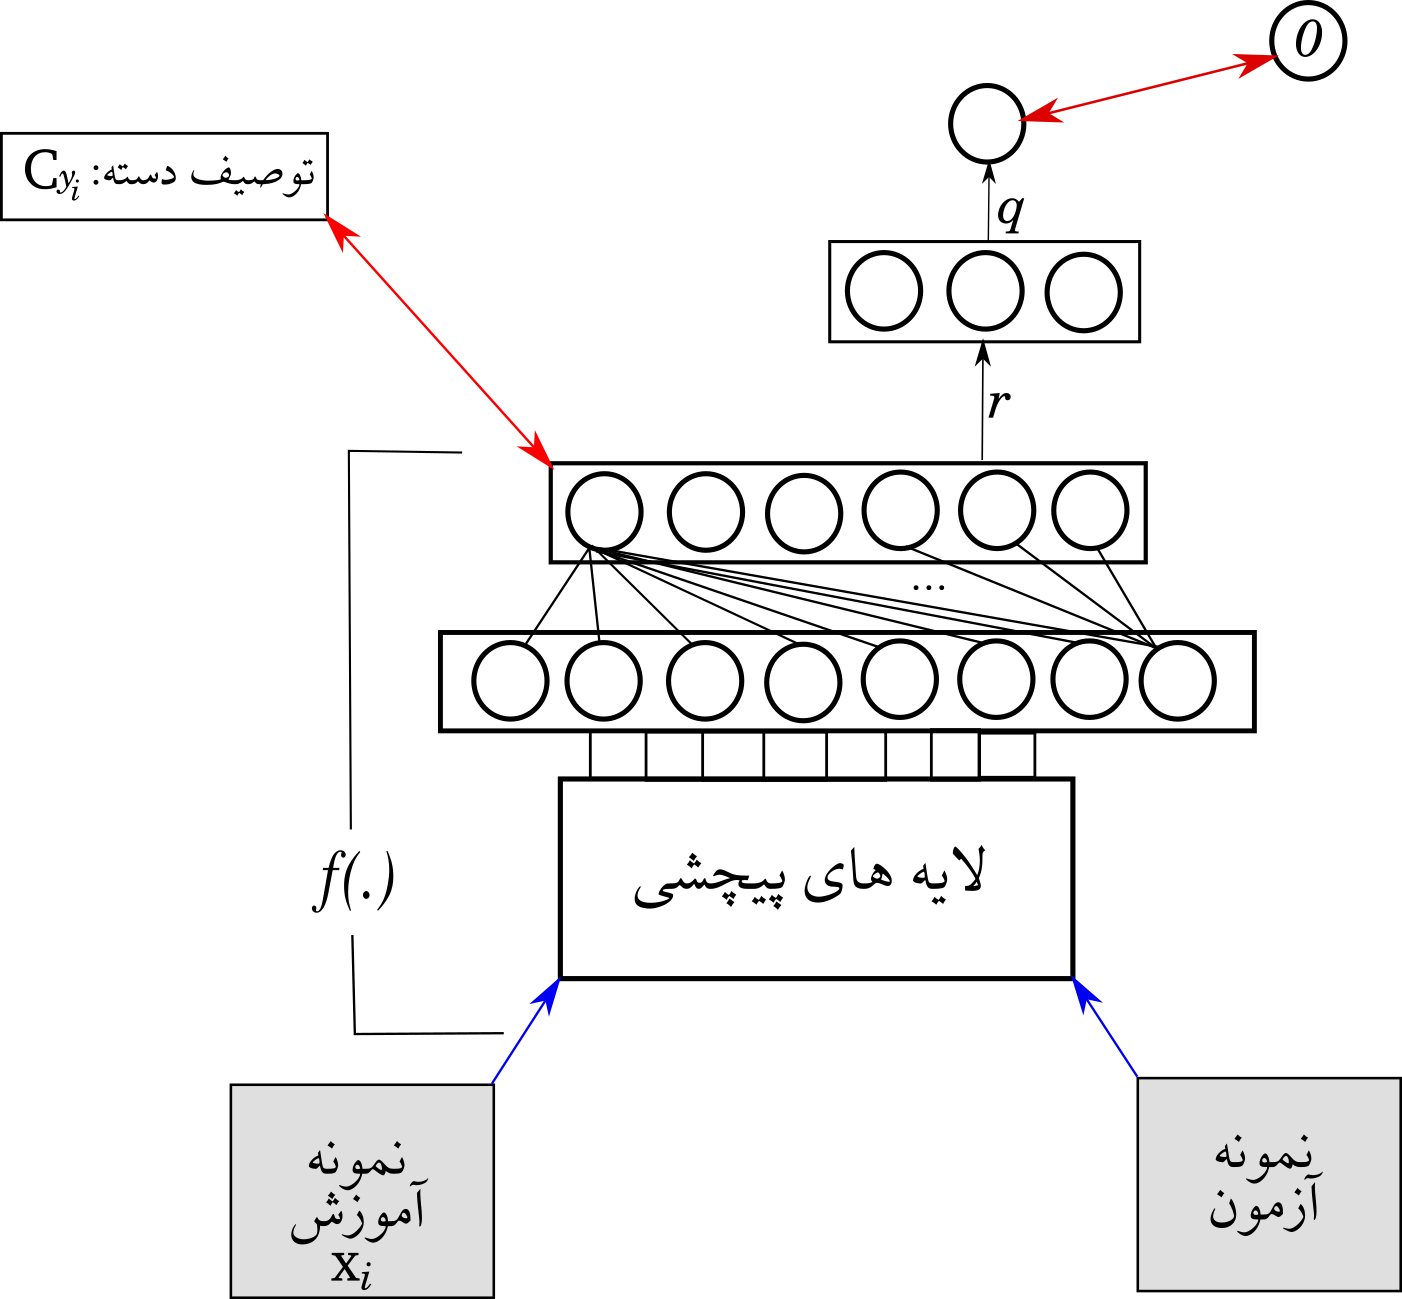
\includegraphics[width=0.85\linewidth]{images/net}
\caption[شبکه‌ی چندوظیفه‌ای پیشنهادی]{
ساختار شبکه چند وظیفه‌ای پیشنهادی. فلش‌های آبی رنگ ورودی‌های شبکه را نشان می‌دهند و فلش‌های قرمز رنگ مقایسه خروجی شبکه با خروجی مورد انتظار را. خطوط سیاه‌رنگ اتصالات شبکه‌ را نشان می‌دهند. زیر شبکه‌ی برگرفته شده از شبکه vgg و یک لایه‌ی با اتصالات چگال اضافه شده بین دو دو ورودی مشترک هستند. لایه‌های $r$ و $q$ مخصوص نمونه‌های آزمون هستند. خروجی لایه‌ی $q$ همواره با مقدار صفر مقایسه می‌شود.
}
\label{fig:nn2}
\end{figure}
یادگیری نگاشت‌ها با استفاده از داده‌های دسته‌های دیده‌شده، همان‌طور که در بخش \ref{lr:semi} اشاره شد، دچار مشکل جابجایی دامنه است و  روی داده‌های دسته‌های دیده‌نشده به خوبی قابل تعمیم نیست. یک راه حل برای مقابله با این مشکل این است که در حین یادیگری نگاشت اجبار شود که حاصل نگاشت یک نمونه‌ی آزمون به نوعی نزدیک به نگاشت توصیف دسته‌های آزمون باشد. همان ‌طور که در بخش
\ref{lr:semi}
بیان شد، چنین راه‌حلی در
\cite{Kodirov2015}
استفاده شده است. معیار نزدیکی نگاشت‌ها در آن روش ه یک امتیاز پیشین از شباهت هر نمونه‌ی آزمون با دسته‌های دیده نشده است که  توسط یک روش دیگر استخراج شده می‌شود. ما در این بخش یک روش مبتنی بر شبکه‌های عصبی عمیق معرفی می‌کنیم که در آن نگاشتی غیرخطی و چندلایه از تصاویر به بردارهای ویژگی یادگرفته می‌شود. یادگیر نگاشت با معیار پیش‌بینی صحیح ویژگی برای نمونه‌های آموزش (که بردار ویژگی صحیح برای آن‌ها مشخص است) و هم‌چنین نزدیک بودن حاصل نگاشت هر نمونه‌ی آزمون به توصیف یکی از دسته‌های دیده نشده است. برای مدل کردن این نگاشت، از یک شبکه‌ی عصبی استفاده شده است. اگر نگاشت مدل شده با شبکه عصبی را با $f$ نشان دهیم، تابع هزینه‌ی مورد استفاده برای آموزش شبکه به صورت زیر تعریف می‌شود:
\begin{equation}
\label{eq:nn_loss}
\min_{f}
\frac{1}{N_s} \sum_{n=1}^{N_s} \normtwo{f(\mathbf{x_i}) - \mathbf{c_{y_i}}} +
\frac{\beta}{N_u} \sum_{i=N_s}^{N_s+N_u} \Big ( \min_{j=n_s,\ldots,n_s + n_u} \normtwo{f(\mathbf{x_i) - c_j}} \Big ),
\end{equation}
که $\beta$ یک فراپارامتر است.
جمله‌ی اول، جمله‌ی مرسوم خطای میانگین مربعات است که در پیش‌بینی مقادیر پیوسته به کار گرفته می‌شود. جمله‌ی دوم برای رفع مشکل جابجایی دامنه طراحی شده است و تحمیل می‌کند که حاصل نگاشت یک نمونه‌ی آزمون حتما نزدیک توصیف یکی از دسته‌های دیده‌نشده باشد، این دسته‌ی دیده نشده، دسته‌ای در نظر گرفته شده است توصیف آن با نگاشت کمترین فاصله را دارد. این انتخاب بر این فرض استوار است که حاصل نگاشت در اکثر موارد به توصیف صحیح نزدیکتر است، یا به عبارتی این که در اکثر مواقع استفاده از دسته‌بند نزدیکترین همسایه روی نگاشتی که تنها با جمله‌ی اول آموزش دیده، دقتی بیش از ۵۰٪ دارد. با این فرض، جمله‌ی دوم این تابع هزینه باعث می‌شود که حاصل روی نمونه‌های آزمون نیز بهتر شود و نگاشته‌شده‌ی هر تصویر فاصله کمتری با توصیف صحیح خود داشته باشد. تابع $\min$ به کاربرده شده در جمله‌دوم معادله
\eqref{eq:nn_loss}
در برخی نقاط مشتق‌پذیر نیست، اما با توجه به اینکه اندازه‌ی این نقاط صفر است تابع تقریبا همه‌جا مشتق‌پذیر است و آموزش شبکه با استفاده از پس‌انتشار\LTRfootnote{back propagation} مقدار گرادیان ممکن خواهد بود. به صورت دقیق‌تر، بهینه‌سازی رابطه \eqref{eq:nn_loss} عملیات محاسبه‌ی مقدار کمینه را داخل شبکه تعبیه می‌کنیم (شکل \ref{fig:nn2})؛ به این صورت که لایه‌های جدید $q$ و$r$ برای نمونه‌های دیده نشده اضافه می‌شود که:
\begin{align}
\label{eq:min_layer}
(q(\mathbf{x}))_j &=  \normtwo{f(\mathbf{v) - c_j}}, \\
r(\mathbf{z}) &= \min_{j=1\ldots n_u} (\mathbf{z})_j.
\end{align}
در هنگام آموزش با پس‌انتشار، مشق تابع هزینه‌ی $l$ نسبت به هر ورودی مثل $z$ در لایه‌ی $r$ با ضابطه‌ی زیر محاسبه می‌شود:
\begin{equation}
\label{eq:grad_min}
\frac{\partial l}{\partial z} = \sum_j \mathds{1}[(z)_j=\min(z)] \cdot \frac{\partial l}{(z)_j)}.
\end{equation}

پس از آموزش شبکه، در فاز آزمون لایه‌های $q$ و $r$ حذف شده و بردار توصیف برای تصاویر آزمون با استفاده از شبکه پیش‌بینی می‌شود، در نهایت دسته‌بندی با استفاده از دسته‌بند نزدیک‌ترین همسایه روی نمونه‌های آزمون انجام خواهد شد:
\begin{equation}
y^{\star}_n = \mathbf{1}_{\argmin_{j} \normtwo{f(\mathbf{x_n - c_j})}}
\end{equation}
\subsection{معماری شبکه}\label{net_architechture}
ما از قسمتی از شبکه‌ی ۱۹ لایه‌ی \lr{vgg} \cite{vgg} که شامل ۱۶ لایه‌ی پیچشی ابتدا و لایه‌‌‌اول با اتصالات چگال به عنوان یک زیر شبکه در ورودی شبکه خود استفاده می‌کنیم. با این زیر شبکه تصاویر ورودی به بردارهای $-4096$بعدی نگاشته می‌شنود. سپس یک لایه‌ی با اتصالات چگال قرار دارد که این حاصل را به بردارهای توصیف دسته‌ها می‌نگارد. سپس برای نمونه‌های آموزش خروجی این لایه با بردار توصیف صحیح مقایسه می‌شود. برای نمونه‌های آزمون خروجی این لایه به  لایه‌های  $q$ و$r$ متصل می‌شود و مقدار خروجی $r$ با مقدار مطلوبش که صفر است مقایسه خواهد شد.
توابع فعال‌سازی در همه‌ی لایه‌ها تابع \lr{ReLU} است که
\begin{equation}
ReLU(\mathbf{x}) = max(\mathbf{0,x}),
\end{equation}
البته در لایه‌ی با اتصالات چگال آخر برای مجموعه‌ دادگانی که مقادیر بردار توصف دودویی هستند از تابع سیگموید برای فعال‌سازی استفاده شده است تا مقادیر در بازه‌ی $[0,1]$ نگاشته شوند.
\section{ تابع مطابقت مبتنی بر خوشه‌بندی }\label{compatibility_funcion}
در اکثر روش‌های پیشین که در فصل \ref{chap:lr} مرور شد، تابع مطابقت میان تصاویر و توصیف‌ها برای اختصاص برچسب به داده‌های آزمون بر اساس فاصله کمینه یا ضرب داخلی بیشینه در یک فضای مشترک محاسبه می‌شد. استثناهای این موضوع، استفاده از روش انتشار برچسب در \cite{Fu2014} و \cite{Kodirov2015} و هم‌چنین پیش‌بینی مستقیم برچسب‌ها در
\cite{li15max}
و
\cite{semi15}
هستند.

\begin{figure}[!t]
\centering
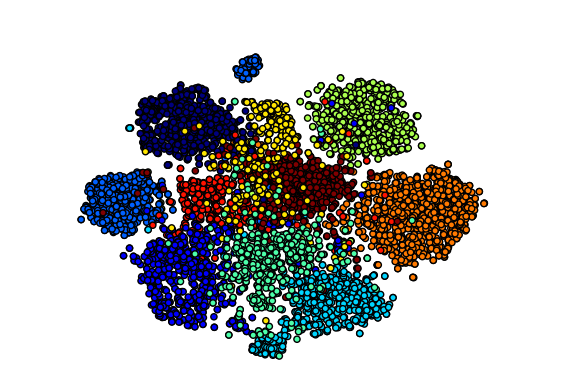
\includegraphics[width=0.85\linewidth]{images/awa_clusters}
\caption[نمایش دسته‌های آزمون مجموعه دادگان AwA ]{
نمایش دوبعدی بوسیله \lr{t-SNE} برای ده دسته‌ی آزمون از مجموعه دادگان AwA با ده رنگ متفاوت نشان داده شده است. درستی فرض قابل خوشه‌بندی در تصویر مشخص است، یعنی ویژگی‌های استخراج شده با استفاده از شبکه‌های عمیق توانایی ایجاد تمایز بالا میان دسته‌ها را دارا هستند.
}
\label{fig:awa_clusters}
\end{figure}

در این بخش ما یک تابع مطابقت جدید بر اساس یک خوشه‌بندی روی داده‌های دسته‌های دیده نشده، تعریف می‌کنیم. اگر فضای نمایش تصاویر دارای این خاصیت باشد که دسته‌های مختلف به صورت خوشه‌های مجزا باشند، استفاده از خوشه‌بندی برای دسته‌بندی برای انتساب برچسب از نظر شهودی توجیه‌پذیر است.
با توجه به نمایش غنی بوجود آمده برای تصاویر توسط شبکه‌های عمیق این فرض در بسیاری از موارد برقرار است. برای نمونه، نمایش \lr{t-SNE} نمونه‌های آزمون مجموعه داده‌های AwA در تصویر
\ref{fig:awa_clusters}
نشان داده شده است و برقراری فرض قابل خوشه‌بندی بودن در آن قابل مشاهده است. این ادعا با استفاده از آزمایش در بخش
\ref{exp:cluster}
اثبات خواهد شد. روش‌های پیشنهادی ما در این فصل بر اساس این ساختار و استفاده از وجود چنین خاصیتی در فضای تصاویر است.
%\section{معرفی یک تابع مطابقت}\label{copatibility_function}
یک راه استفاده از چنین خاصیتی در فضای تصاویر، معرفی یک تابع مطابقت است که علاوه بر شباهت نگاشت‌یافته‌ی نمونه‌ها و توصیف‌ها به سایر نمونه‌های در همسایگی هر نمونه نیز وابسته باشد. بدین منظور ما یک تابع مطابقت جدید پیشنهاد می‌دهیم که در آن برچسب تعلق گرفته به هر نمونه به نمونه‌هایی که با آن‌ها در یک خوشه قرار گرفته است وابسته است. به این منظور ابتدا باید یک خوشه‌بندی روی نمونه‌ها انجام شود سپس با استفاده از یک معیار (که یک نمونه از آن را در بخش \ref{simple_method} معرفی می‌کنیم) میزان شباهت خوشه به توصیف تعیین می‌شود. این در مقابل حالتی است که تابع مطابقت میزان شباهت تک تک نمونه‌ها را توصیف‌ها محاسبه می‌کرد.
 در این حالت هر خوشه باید یک برچسب دریافت کند و برچسب اختصاص یافته به هر خوشه، توسط تمام اعضای آن به ارث برده می‌شود. این تابع مطابقت تا کنون در روش‌های موجود برای یادگیری بدون برد استفاده نشده بوده است. این تابع مطابقت قابل اضافه شدن به روش‌های دیگر نیز می‌باشد. به این صورت که پیش‌بینی‌های انجام شده در آن روش را در نظر گرفته و با استفاده از آن‌ها در هر خوشه رای‌گیری انجام دهیم تا برچسبی که کل خوشه دریافت می‌کند تعیین شود. آزمایش‌ها نشان می‌دهند که  اضافه شدن این تابع مطابقت عمل‌کرد روش‌های پایه را بهبود می‌دهد.
%-----------------------------------------------------------Section -----------
\section{یک خوشه‌بندی نیمه‌نظارتی}\label{clustering_method}
عمل‌کرد تابع مطابقت معرفی شده در بخش قبل وابسته به دقت خوشه‌بندی انجام شده روی داده‌هاست. در واقع دقت خوشه‌بندی انجام شده، حد بالای دقت نهایی روش خواهد بود و این در حالتی رخ می‌دهد که هر خوشه برچسبی را دریافت کند که برچسب صحیح  اکثر اعضای آن است. با توجه به این موضوع وجود یک خوشه‌بندی دقیق برای استفاده از این تابع مطابقت ضروری است. البته در آزمایش‌های انجام شده، با استفاده از  الگوریتم خوشه‌بندی
\lr{k-means} \cite{kmeans}
نیز می‌توان به عمل‌کرد پیشگام دست پیدا کند. اما این الگوریتم در خوشه‌بندی نمونه‌های آزمون استفاده‌ای از برچسب‌هایی که برای نمونه‌های آموزش وجود دارد، نخواهد کرد و این اطلاعات می‌توان باعث بهبود عمل‌کرد خوشه‌بندی شود. از طرفی الگوریتم‌های نیمه‌نظارتی موجود برای خوشه‌بندی نیز بر مسئله یادگیری بدون برد تطابق ندارند. در حالت معمول یادگیری نیمه‌نظارتی \cite{chapel06}، مسئله به این صورت تعریف می‌شود که داده‌های برچسب‌دار و بدون برچسب همگی به یک مجموعه دسته‌ی یکسان تعلق دارند و داده‌های بدون برچسب نیز در نهایت برچسب یکسانی با داده‌های برچسب‌دار دریافت می‌کنند. این در حالی‌ست که در مسئله یادگیری بدون برد، نمونه‌های بدون برچسب در دسته‌های مجزا از نمونه‌های برچسب‌دار قرار می‌گیرند. با توجه به این موضوع، یک روش خوشه‌بندی نیمه‌نظارتی پیشنهاد می‌کنیم که با فرض‌های مسئله یادگیری بدون برد منطبق باشد. در این روش خوشه‌بندی همانند k-means عمل می‌شود با این تفاوت که اگر شماره خوشه نمونه‌های دیده شده  برابر با برچسب صحیح آن‌ها نباشد، جریمه‌ای در نظر گرفته می‌شود. تابع هزینه این روش به این صورت تعریف شده است:
\begin{equation} \label{eq:my_clustering}
\min_{R, \boldsymbol{\mu_1, \ldots, \mu_k }}  \sum_{n,k} r_{nk} \normtwo{\mathbf{x_n} - \boldsymbol{\mu_k}} +
 \beta \sum_{n=1}^{N_s} \mathds{1}(\mathbf{r_n} \neq \mathbf{y_n}),
\end{equation}
در این معادله $ \boldsymbol{\mu_1, \ldots, \mu_k }$ مراکز خوشه‌ها و $R$ ماتریس اختصاص داده‌ها خوشه‌هاست، جمله اول همان جمله موجود در تابع هزینه‌ی
\lr{k-means}
است. علاوه بر این، در جمله‌ی دوم برای هر نمونه‌ی برچسب‌دار، اگر به خوشه‌ای تعلق بگیرد که شماره آن با برچسبش متفاوت باشد، جریمه $\beta$ در نظر گرفته می‌شود. در نتیجه این روش، $n_s$ خوشه ابتدایی را به سمت این سوق می‌دهند که همان $n_s$ دسته‌ی دیده شده باشند.  $\beta$ یک فراپارامتر مدل است که اهمیت این جمله اضافه شده را تعیین می‌کند.


% فرض کنید که نمونه‌های $X_u$ با یک روش خوشه‌بندی به $n_u$ خوشه تقسیم شده‌اند و $R$ ماتریس اختصاص خوشه‌ها با نمایش یکی‌یک است.
\section{روش دسته‌بندی مبتنی بر خوشه‌بندی} \label{simple_method}
در این بخش روشی معرفی می‌شود که همراه با خوشه‌بندی بخش قبل یک چارچوب برای دسته‌بندی در مسئله یادگیری بدون برد را تشکیل می‌دهند. برای نسبت دادن برچسب به خوشه‌ها، به دنبال یافتن نمایشی از امضای هر دسته در فضای تصاویر به عنوان نماینده آن دسته در فضای تصاویر هستیم. از نظر شهودی مطلوب است که این نماینده‌ها بر مرکز خوشه‌هایی که در فضای تصاویر تشکیل می‌شود منطبق باشند. برای محقق شدن این خاصیت، نگاشت را به صورتی یاد می‌گیریم که حاصل نگاشت توصیف دسته‌های آموزش منطبق بر میانگین نمونه‌های این دسته‌ها باشد:
\begin{equation} \label{eq:d_definition}
  D = \argmin_D \normf{X_s - D Z_s}^2 + \gamma \normf{D}^2,
\end{equation}
در این معادله، ستون‌های
 $Z_s \in \mathbb{R}^{a \times N_s}$
  امضای دسته‌های نمونه‌های $X_s$ هستند و $\gamma$ یک فراپارامتر است که با اعتبارسنجی تعیین خواهد شد. مسئله تعریف شده برای یافتن نگاشت $D$، امضای کلاس را طوری می‌نگارد که نزدیک به مرکز نمونه‌های آن دسته باشد و این در حالت ایده‌آل همان مرکز خوشه‌ها خواهد بود. در نتیجه این نگاشت برای تعیین دسته‌ها به صورت نزدیک‌ترین همسایه مطلوب بنظر می‌رسد. مسئله بهینه‌سازی
  \eqref{eq:d_definition}
  دارای جواب فرم بسته‌ی زیر است:
  \begin{equation} \label{eq:d_answer}
  D = X_s Z_s^T (Z_s Z_s^T + \gamma I)^{-1}.
\end{equation}

برای تخصیص برچسب به هر خوشه از این رابطه استفاده می‌کنیم:
\begin{equation}
\label{eq:simple_assignment}
\ell(\boldsymbol{\mu_k}) = \argmin_{u=1,\ldots,n_u} \normf{\boldsymbol{\mu_k} - DC_{s(u)}}^2
\end{equation}
و تمامی عناصر خوشه‌ی $k$م برچسب $\ell(\boldsymbol{\mu_k})$ را دریافت می‌کنند.

در این روش سه فراپارامتر وجود دارد، یک پارامتر $\gamma$ در معادله
\eqref{eq:d_definition}
است و دو پارامتر دیگر که مربوط به خوشه‌بندی نیمه‌نظارتی هستند، یعنی $k$ و $\beta$ در معادله
\eqref{eq:my_clustering}.
در آزمایش‌ها عملی دریافتیم که روش به مقدار پارامتر $\gamma$ حساس است در نتیجه مقدار آن توسط یک روند اعتبارسنجی تعیین خواهد شد، نحوه‌ی اعتبارسنجی به صورت دقیق در بخش
\ref{exp:validation}
بیان خواهد شد. در مقابل، مدل به پارامترهای $k$ و $\beta$ حساس نبود، در نتیجه برای ساده و سریع‌تر شدن روند آموزش مقدار آن‌ها را ثابت در نظر گرفته‌ایم. برای $k$ مقدار
$k = n_s + 2n_u$
در نظر گرفته شده است تا هر کدام از دسته‌های دیده‌نشده بتوانند با دو خوشه نمایش داده شوند و در نتیجه پراکندگی و اختلاف میان نمونه‌های یک دسته پوشش داده شود. مقدار $\beta$ نیز در حالتی که داده‌ها به صورت $\norm{x}_1=1$ نرمال شده‌اند، برابر $1$ در نظر گرفته شده است.
در آزمایش‌ها عملی که در فصل
\ref{chap:experiments}
گزارش می‌شود، مشاهده می‌شود که این روش  عمل‌کرد پیشگام در دقت دسته‌بندی بدون برد را روی سه مجموعه دادگان از چهار مجموعه بهبود می‌بخشد.

\subsection{بهینه‌سازی}\label{simple_opt}
 کمینه‌کردن تابع هزینه معرفی شده در رابطه
\eqref{eq:my_clustering}،
با توجه به این که $R$ یک افراز\LTRfootnote{partitioning} روی نمونه‌هاست، مانند بهینه‌سازی تابع هزینه‌ی \lr{k-means} یک مسئله‌ی \nphard است \cite{kmeans_nphard}. در نتیجه ما از یک تقریب
مشابه الگوریتم خوشه‌بندی \lr{k-means} استفاده می‌کنیم که یک بهینه محلی برای این تابع را پیدا می‌کند. به این منظور،  یک روند تناوبی\LTRfootnote{alternative}  میان بهینه کردن بر اساس $R$ و $\mu_k$ها به کار گرفته می‌شود. برای بروز رسانی $\mu_k$ روی اعضای خوشه $k$ میانگین گرفته می‌شود:
\begin{equation} \label{eq:updata_mu}
 \boldsymbol{\mu_k} = \frac{\sum_{n=1}^{N_s + N_u}  \mathds{1}(r_{nk}=1)\mathbf{x_n}}{\sum_{n=1}^{N_s+N_u}\mathds{1}(r_{nk}=1)}.
\end{equation}
برای بروز رسانی $R$ هر نمونه به خوشه‌ای اختصاص می‌یابد که کمترین فاصله را با مرکز آن دارد:
\begin{equation} \label{eq:updata_R}
R_{(n)} = \mathbf{1_{\argmin_k \normtwo{x_n - \mu_k}}}, \quad n=1,\ldots,N_s+N_u
\end{equation}
برای مقداردهی اولیه به $\mu_k$ برای  خوشه‌های مربوط به دسته‌های دیده شده، میانگین عناصر آن‌ها را قرار می‌دهیم:
\begin{equation} \label{eq:init_mu}
 \boldsymbol{\mu_k^0} = \frac{\sum_{n=1}^{N_s + N_u}  \mathds{1}(Y_{s(n)} = \mathbf{1_k})\cdot \mathbf{x_n}}{\sum_{n=1}^{N_s+N_u}\mathds{1}(Y_{s(n)} = \mathbf{1_k})},
\quad 1 \leq k \leq n_s
\end{equation}
برای سایر خوشه‌ها، یعنی خوشه‌های مربوط به دسته‌های دیده نشده از الگوریتم
\lr{k-means++ } \cite{kmeanspp}
استفاده می‌کنیم.
روند کامل این روش دسته‌بندی در الگوریتم
\ref{alg:simple}
بیان شده است.

\شروع{program}
	\begin{enumerate}[label={\arabic*},itemsep=.1em, parsep=.1em]
\فقره {\bf ورودی:} تصاویر و توصیف‌های آموزش و آزمون و برچسب‌های نمونه‌های آموزش $X_s, X_u, Y_s, Z_s, C_u$
\فقره {\bf خروجی:} برچسب‌های پیش‌بینی شده برای نمونه‌های آزمون:$Y_u$
\فقره   $k \in \{ 1,2, \ldots, n_s + n_u \}$
\فقره  $n \in \{ 1,2, \ldots, N_s + N_u \}$
\فقره  $\boldsymbol{\mu_k}$ را برای  $k=1,\ldots,n_s$،  با رابطه \eqref{eq:init_mu} مقداردهی کن.
\فقره  $\boldsymbol{\mu_k}$ را برای $k=n_s+1,\ldots,n_s+n_u$، با استفاده از \lr{k-means++} مقداردهی کن.
\فقره تا همگرایی به یک بهینه‌ی محلی، موارد زیر را تکرار کن

\فقره
 $\qquad$   $ a_n \leftarrow  {\argmin_i \lVert x_n - \mu_i \rVert_2}$ //تخصیص خوشه‌ها
\فقره
 $\qquad$ $\mathbf{\mu_k} \leftarrow \sum_{n} \mathbf{x_n} \mathds{1}(a_n = k) / \sum_n (\mathds{1}(a_n = k) $

\فقره  $  D \leftarrow X_s Y_s^T (Y_s Y_s^T + \gamma I)^{-1}$
\فقره  $l[k] \leftarrow \argmin_j \lVert \mathbf{\mu_k} - (DS_u)_{(j)} \rVert_2$
\فقره   $\mathbf{(Y_u)_{(n)}} \leftarrow \mathbf{1}_{l[a_n]}$
\فقره $Y_u$ را برگردان
\end{enumerate}
\caption{الگوریتم ساده خوشه‌بندی و دسته‌بندی با تابع مطابقت پیشنهاد شده}
\label{alg:simple}
\پایان{program}


%-------------------------------------------------- section
\section{خوشه‌بندی و نگاشت توام} \label{jeac}
روش ارائه شده در فصل قبل، هر چند که به دقت دسته‌بندی بالاتری از روش‌های پیشین دست پیدا می‌کند اما دقت دسته‌بندی در آن توسط دقت خوشه‌بندی صورت گرفته محدود شده است. برای حل این معضل در این روش یک چارچوب معرفی می‌کنیم که خوشه‌بندی و نگاشت توصیف دسته‌ها به فضای تصاویر در آن به صورت توام انجام شود.
برای این منظور تابع هزینه‌ی زیر پیشنهاد می‌شود:
\begin{align}
\label{eq:joint}
 \min_{R,D} \normf{X_s - D Z_s}^2  &+ \lambda \normf{X_u - D C_u R^T }^2 + \gamma \normf{D}^2 \\
   s.t. \quad & R \in \{0,1\}^{N_u \times n_u}. \nonumber
\end{align}
در این معادله $\gamma$ و $\lambda$ فراپارامترهای مدل هستند. جمله اول و سوم در رابطه بالا مشابه رابطه \eqref{eq:d_definition} هستند و تاثیر آن‌ها همانند حالت قبل این است که نگاشت $D$ بتواند امضای دسته‌های دیده نشده را به مرکز تصاویر هر دسته بنگارد. جمله دوم که در این معادله اضافه شده، ذاتا یک جمله خوشه‌بندی است. اگر جمله دوم در عبارت بالا را از فرم ماتریسی خارج کرده و بر حسب عناصر $R$ بیان کنیم این مسئله واضح‌تر  خواهد شد:
\begin{equation}
\label{eq:essentialy_clustering}
\sum_{n=N_s+1}^{N_s + N_u} \sum_{k=1}^{n_u} r_{nk} \normtwo{\mathbf{x_n} - D \mathbf{c_k}},
\end{equation}
که مشابه تابع هزینه‌ی
\lr{k-means}
است، با این تفاوت که مراکز خوشه‌ها کاملا آزاد نیستند بلکه مراکز خوشه‌ها باید تصویر امضای دسته‌های دیده نشده باشد که توسط نگاشت $D$ به فضای تصاویر نگاشته شده است. در این حالت برچسب‌های پیش‌بینی شده برای نمونه‌ها همان انتساب‌های آن‌ها به خوشه‌هاست که در طول جریان آموزش توامان با نگاشت $D$ یادگرفته می‌شود. در نتیجه مشکل بیان شده برای روش قبل، در این چهاچوب وجود ندارد. جمله خوشه‌بندی را در این چارچوب می‌توان به این صورت نیز تعبیر کرد که این جمله یادگیری نگاشت $D$ را به صورتی بهبود می‌دهد که مشکل جابجایی دامنه در آن وجود نداشته باشد. در حالت عادی برای یادگیری نگاشت $D$ توسط رابطه
\eqref{eq:d_definition}
تنها از نمونه‌های آموزش برای یافتن $D$ استفاده می‌شد، در نتیجه مشکل جابجایی دامنه برای داده‌های آزمون بوجود می‌آمد، چرا که این داده‌ها در تعیین نگاشت $D$ بی‌تاثیر بوده‌اند. اما جمله اضافه شده در چارچوب فوق الزام می‌کند که امضای هر دسته‌ی دیده نشده نزدیک به تعدادی از داده‌های آزمون (که توسط $R$ مشخص می‌شوند) نگاشته شود. این مسئله می‌تواند مانع از مشکل جابجایی دامنه شود. این موضوع در بخش
\ref{exp:discussion}
بیشتر بررسی خواهد شد.
\subsection{بهینه‌سازی}

\شروع{program}[t!]
	\begin{enumerate}[label={\arabic*},itemsep=.1em, parsep=.1em]
\فقره {\bf ورودی:} تصاویر و توصیف‌های آموزش و آزمون و برچسب‌های نمونه‌های آموزش $X_s, X_u, Y_s, Z_s, C_u$
\فقره {\bf خروجی:} برچسب‌های پیش‌بینی شده برای نمونه‌های آزمون:$R$
\فقره $R$ را با خروجی الگوریتم \ref{alg:simple} مقدار دهی کن.
\فقره تا هنگامی که مقدار $R$ تغییر نکند،  تکرار کن:
\فقره $\qquad$  $D$ را با رابطه \eqref{eq:joint_d_update} بروزرسانی کن.
\فقره $\qquad$ عناصر $R$ را با استفاده از رابطه \eqref{eq:joint_r_update} بروزرسانی کن.
\فقره $R$ را برگردان
\end{enumerate}
\caption{الگوریتم یادگیری نگاشت و خوشه‌بندی به صورت توام}
\label{alg:jeac}
\پایان{program}

مسئله بهینه‌سازی رابطه \eqref{eq:joint} بر حسب هر دو متغیر $R$ و $D$ محدب\LTRfootnote{convex}  نیست اما بر حسب هر کدام از آن‌ها به تنهایی، محدب است. در نتیجه برای یافتن یک بهینه محلی از یک روند تناوبی میان بهینه‌کردن بر حسب $R$ و $D$ استفاده می‌کنیم.
برای بروز رسانی $D$ جواب به فرم بسته وجود دارد:
\begin{equation} \label{eq:joint_d_update}
  D = (X_s Z_s^T + \beta X_u R C_u^T) (Z_s Z_s^T + \beta C_u R^T R C_u^T  + \gamma I)^{-1},
\end{equation}
و مقدار بهینه برای $R$، زمانی که $D$ ثابت باشد، با نسبت دادن هر نمونه به نزدیک‌ترین مرکز خوشه به دست می‌آید:
\begin{equation} \label{eq:joint_r_update}
  r_{ij} = \mathds{1}[j = \argmin_{k} \lVert X_{u(i)} - D S_{u(k)} \rVert_2 ].
\end{equation}
در این روند بین بروز رسانی $D$ و $R$ تناوب انجام می‌شود تا جایی که $R$ ثابت بماند یعنی تغییری در برچسب‌های پیش‌بینی شده برای هیچ‌کدام از نمونه‌ها رخ ندهد. در آزمایش‌ها انجام شده این همگرایی همواره در کمتر از ۲۰ بار بروز رسانی به دست می‌آید.
مراحل این روش در الگوریتم \ref{alg:jeac} آمده است.
\section{جمع‌بندی}
در این بخش ابتدا یک شبکه عصبی برای انجام پیش‌بینی ویژگی در مسئله یادگیری بدون برد ارائه شد. پس از آن یک تابع مطابقت جدید برای مسئله یادگیری بدون برد ارائه شد. برای بهره‌گیری مناسب از این تابع مطابقت یک خوشه‌بندی دقیق روی نمونه‌های آزمون مورد نیاز بود. به این خاطر، سپس یک الگوریتم خوشه‌بندی نیمه‌نظارتی که با فرض‌های مسئله‌ی یادگیری بدون برد هم‌خوانی داشته باشد ارائه گردید. یک چارچوب برای دسته‌بندی بدون برد با استفاده از تابع مطابقت و خوشه‌بندی پیشنهادی و یک نگاشت خطی از فضای توصیف دسته‌ها به فضای تصاویر ارائه شد. بعد از آن یک روش که یادیگری نگاشت و خوشه‌بندی در آن  به صورت توام انجام شود ارائه شد و در مورد نحوه‌ی بهینه‌سازی توابع پیشنهادی در این روش‌ها بحث شد.
%--------------------------section
